\documentclass{bmcart}

%%%%%%%%%%%%%%%%%%%%%%%%%%%%%%%%%%%%%%%%%%%%%%
%%                                          %%
%% CARGA DE PAQUETES DE LATEX               %%
%%                                          %%
%%%%%%%%%%%%%%%%%%%%%%%%%%%%%%%%%%%%%%%%%%%%%%

%%% Load packages
\usepackage{amsthm,amsmath}
\usepackage{graphicx}
%\RequirePackage[numbers]{natbib}
%\RequirePackage{hyperref}
\usepackage{hyperref}
\usepackage[utf8]{inputenc} %unicode support
%\usepackage[applemac]{inputenc} %applemac support if unicode package fails
%\usepackage[latin1]{inputenc} %UNIX support if unicode package fails
\usepackage{tabularx} 
\usepackage{array} 
%%%%%%%%%%%%%%%%%%%%%%%%%%%%%%%%%%%%%%%%%%%%%%
%%                                          %%
%% COMIENZO DEL DOCUMENTO                   %%
%%                                          %%
%%%%%%%%%%%%%%%%%%%%%%%%%%%%%%%%%%%%%%%%%%%%%%

\begin{document}

	\begin{frontmatter}
	
		\begin{fmbox}
			\dochead{Research}
			
			%%%%%%%%%%%%%%%%%%%%%%%%%%%%%%%%%%%%%%%%%%%%%%
			%% INTRODUCIR TITULO PROYECTO               %%
			%%%%%%%%%%%%%%%%%%%%%%%%%%%%%%%%%%%%%%%%%%%%%%
			
			\title{Hoffmann's sign}
			
			%%%%%%%%%%%%%%%%%%%%%%%%%%%%%%%%%%%%%%%%%%%%%%
			%% AUTORES. METER UNA ENTRADA AUTHOR        %%
			%% POR PERSONA                              %%
			%%%%%%%%%%%%%%%%%%%%%%%%%%%%%%%%%%%%%%%%%%%%%%
			
			\author[
			  addressref={aff1},                   % ESTA LINEA SE COPIA IGUAL PARA CADA AUTOR
			  corref={aff1},                       % ESTA LINEA SOLO DEBE TENERLA EL COORDINADOR DEL GRUPO
			  email={jane.e.doe@cambridge.co.uk}   % VUESTRO CORREO ACTIVO
			]{\inits{J.E.}\fnm{Jane E.} \snm{Doe}} % inits: INICIALES DE AUTOR, fnm: NOMBRE DE AUTOR, snm: APELLIDOS DE AUTOR
			\author[
			  addressref={aff1},
			  email={alexsilva@uma.es}
			]{\inits{A.S.R.}\fnm{Alejandro} \snm{Silva Rodríguez}}
			
			\author[
			addressref={aff1},
			email={0610948742@uma.es} 
			]{\inits{J.I.S.M.}\fnm{Juan Ignacio} \snm{Soriano Muñoz}}
			
			%%%%%%%%%%%%%%%%%%%%%%%%%%%%%%%%%%%%%%%%%%%%%%
			%% AFILIACION. NO TOCAR                     %%
			%%%%%%%%%%%%%%%%%%%%%%%%%%%%%%%%%%%%%%%%%%%%%%
			
			\address[id=aff1]{%                           % unique id
			  \orgdiv{ETSI Informática},             % department, if any
			  \orgname{Universidad de Málaga},          % university, etc
			  \city{Málaga},                              % city
			  \cny{España}                                    % country
			}
		
		\end{fmbox}% comment this for two column layout
		
		\begin{abstractbox}
		
			\begin{abstract} % abstract
			
			%%%%%%%%%%%%%%%%%%%%%%%%%%%%%%%%%%%%%%%%%%%%%%%
			%% RESUMEN BREVE DE NO MAS DE 100 PALABRAS   %%
			%%%%%%%%%%%%%%%%%%%%%%%%%%%%%%%%%%%%%%%%%%%%%%%	
			
			\end{abstract}
			
			%%%%%%%%%%%%%%%%%%%%%%%%%%%%%%%%%%%%%%%%%%%%%%
			%% PALABRAS CLAVE DEL PROYECTO              %%
			%%%%%%%%%%%%%%%%%%%%%%%%%%%%%%%%%%%%%%%%%%%%%%
			
			\begin{keyword}
			\kwd{sample}
			\kwd{article}
			\kwd{author}
			\end{keyword}
		
		
		\end{abstractbox}
	
	\end{frontmatter}
	
	%%%%%%%%%%%%%%%%%%%%%%%%%%%%%%%%%%%%%%%%%%%%%%%%%%%%%%%%%%%%%%%%%%%%%%%%%%%%%%%%%%%%%%%%
	%% EJEMPLO DE LATEX %%                                                                %%
	%% BORRAR ANTES DE ENTREGAR!!!!!!!!!!!!!!!!!!!!!!!!!!!!!!!!!!!!!!!!!!!!!              %%
	%%%%%%%%%%%%%%%%%%%%%%%%%%%%%%%%%%%%%%%%%%%%%%%%%%%%%%%%%%%%%%%%%%%%%%%%%%%%%%%%%%%%%%%%
	
	\section*{Content}
		Text and results for this section, as per the individual journal's instructions for authors. Here, we reference the figure xd but also the table \ref{tab:ejemplo}.
	
	\section*{Section title}
		Text for this section\ldots

		In this section we examine the growth rate of the mean of $Z_0$, $Z_1$ and $Z_2$. In
		addition, we examine a common modeling assumption and note the
		importance of considering the tails of the extinction time $T_x$ in
		studies of escape dynamics.
		We will first consider the expected resistant population at $vT_x$ for
		some $v>0$, (and temporarily assume $\alpha=0$)
		%
		\[
		E \bigl[Z_1(vT_x) \bigr]=
		\int_0^{v\wedge
			1}Z_0(uT_x)
		\exp (\lambda_1)\,du .
		\]
		%
		If we assume that sensitive cells follow a deterministic decay
		$Z_0(t)=xe^{\lambda_0 t}$ and approximate their extinction time as
		$T_x\approx-\frac{1}{\lambda_0}\log x$, then we can heuristically
		estimate the expected value as
		%
		\begin{equation}\label{eqexpmuts}
			\begin{aligned}[b]
				&      E\bigl[Z_1(vT_x)\bigr]\\
				&\quad      = \frac{\mu}{r}\log x
				\int_0^{v\wedge1}x^{1-u}x^{({\lambda_1}/{r})(v-u)}\,du .
			\end{aligned}
		\end{equation}
		%
		%%%%%%%%%%%%%%%%%%%%%%%%%%%%%%%%%%%%%%%%%%%%%%%%%%%%%%%%%%%%%%%%%%%%%%
		%% USAR \cite{...} PARA INCLUIR REFERENCIAS BIBLIOGRAFICAS          %%
		%%  \cite{koon}  Para una sola                                      %%
		%%  \cite{oreg,khar,zvai,xjon,schn,pond} Para una lista             %%
		%%%%%%%%%%%%%%%%%%%%%%%%%%%%%%%%%%%%%%%%%%%%%%%%%%%%%%%%%%%%%%%%%%%%%%
		Thus we observe that this expected value is finite for all $v>0$
		
		
		%%%%%%%%%%%%%%%%%%%%%%%%%%%%%%%%%%%%%%%%%%%%%%%%%%%%%%%%%%%%%%%%%%%%%%%%%%%%%%%%%%%%%%%%%%%
		%% FIGURAS                                                                               %%
		%% includegraphics: inserta la imagen                                                    %%
		%% caption: descripcion de la figura                                                     %%
		%% label: etiqueta para hacer referencia a la figura en el texto con la instrucción ref  %%
		%%%%%%%%%%%%%%%%%%%%%%%%%%%%%%%%%%%%%%%%%%%%%%%%%%%%%%%%%%%%%%%%%%%%%%%%%%%%%%%%%%%%%%%%%%%	
		%%%%%%%%%%%%%%%%%%%%%%%%%%%%%%%%%%%%%%%%%%%%%%%%%%%%%%%%%%%%%%%%%%%%%%%%%%%%%%%%%%%%%%%%%%
		%% TABLAS                                                                               %%
		%% caption: Descripción tabla                                                           %%
		%% \begin{tabular}{letras}: Indica numero de columnas.                                  %%
		%%    Una letra por columna, la letra indica la alineación de la columna:               %%
		%%    c center, l left, r right                                                         %%
		%% hline: Representa una linea como entre filas                                         %%
		%% \\: fin de fila                                                                      %%
		%% &: delimitador de celda                                                              %%
		%% label: etiqueta para hacer referencia a la tabla en el texto con la instrucción ref  %%
		%%%%%%%%%%%%%%%%%%%%%%%%%%%%%%%%%%%%%%%%%%%%%%%%%%%%%%%%%%%%%%%%%%%%%%%%%%%%%%%%%%%%%%%%%%
		
		\begin{table}[h!]
			\caption{Sample table title. This is where the description of the table should go}
			\begin{tabular}{cccc}
				\hline
				& B1  &B2   & B3\\ 
				\hline
				A1 & 0.1 & 0.2 & 0.3\\
				A2 & ... & ..  & .\\
				A3 & ..  & .   & .\\ 
				\hline
				\label{tab:ejemplo}
			\end{tabular}
		\end{table}
				
		\subsection*{Sub-heading for section}
			Text for this sub-heading\ldots
	
			\subsubsection*{Sub-sub heading for section}
				Text for this sub-sub-heading\ldots
					
					\paragraph*{Sub-sub-sub heading for section}
						Text for this sub-sub-sub-heading\ldots
	
	%%%%%%%%%%%%%%%%%%%%%%%%%%%%%%%%%
	%% FIN DE EJEMPLO !!!!!!!!!!!! %%
	%%%%%%%%%%%%%%%%%%%%%%%%%%%%%%%%%
	
	%%%%%%%%%%%%%%%%%%%%%%%%%%%%%%%%%
	%% COMIENZO DEL DOCUMENTO REAL %%
	%%%%%%%%%%%%%%%%%%%%%%%%%%%%%%%%%
	
	\section{Introducción}
El signo de Hoffmann es un reflejo muscular que se produce al percutir suavemente el lecho ungueal del dedo medio o índice como se muestra en la figura \ref{fig:Hoffman_sign}, produciéndose un movimiento de flexión involuntario del pulgar cuando el examinador hace girar la uña del dedo medio hacia abajo. Fue propuesto por primera vez por Johann Hoffmann, un neurólogo alemán, a finales del siglo XIX. Y descrito por primera vez gracias a Hans Curschmann, uno de sus asistentes, en 1911\cite{ BENDHEIM}. El signo de Hoffmann también ha sido denominado de diferentes formas, como "reflejo digital", "reflejo de chasquido", "signo de Tromner" y "signo de Jakobson" \cite{glaser2001cervical}.


\begin{figure}[h!]
	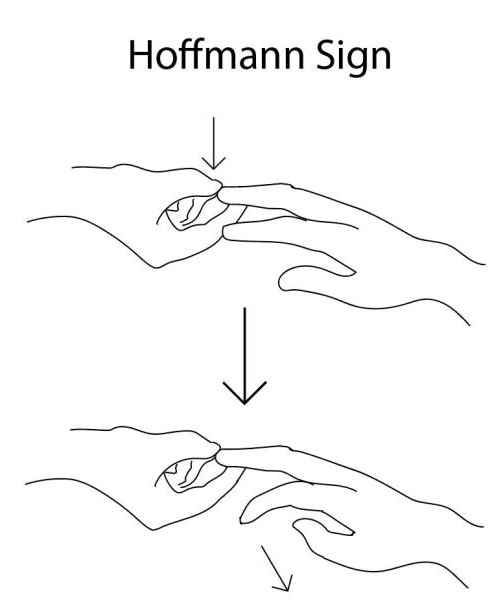
\includegraphics[width=0.35\textwidth]{figures/Kabir_Hoffmann__Sign.jpg}
	\caption{Signo de Hoffmann. Este diagrama muestra un signo de Hoffmann positivo, una parte estándar del examen neurológico común. Contribución de R Kabir, MD}
	\label{fig:Hoffman_sign}
\end{figure}

Se ha utilizado en la práctica clínica durante aproximadamente cien años como una herramienta para detectar alteraciones en las vías corticoespinales, las cuales conectan la corteza cerebral con la médula espinal. Estudios realizados en la década de 1930 evaluaron la incidencia del signo en estudiantes universitarios sanos, encontrando una incidencia del 2\% y 1.63\% \cite{echols1936hoffmann} \cite{fay1933clinical} respectivamente, aunque solo se incluyeron sujetos masculinos \cite{glaser2001cervical}. Este hallazgo clínico ha sido útil en la detección de mielopatía cervical espondilótica temprana \cite{denno1991early}, como lo propusieron Denno y Meadows al describir el signo de Hoffmann "dinámico", una variante de la prueba con flexiones activas del cuello \cite{glaser2001cervical}.

Es importante destacar que el signo de Hoffman es un fenotipo y no una enfermedad en sí, se ha descubierto que hasta el 3\% de la población presenta un signo de Hoffmann positivo sin que haya compresión de la médula. Este reflejo está asociado a 12 enfermedades diferentes\cite{whitney}.

El signo de Hoffmann ha sido identificado en una serie de enfermedades neurodegenerativas y trastornos del tracto corticoespinal, muchas de ellas caracterizadas por alteraciones motoras progresivas. Entre estas patologías se encuentran diversas formas de paraplejía espástica hereditaria, son un grupo clínicamente y genéticamente heterogéneo de trastornos neurológicos, caracterizados principalmente por espasticidad progresiva y, a menudo, pérdida del sentido de la vibración en los miembros inferiores \cite{Esteves2014}, tanto autosómica dominante como recesiva. Por ejemplo, la paraplejía espástica 9A, de herencia autosómica dominante (OMIM:601162) \cite{10.1093/brain/awv143}, y las formas recesivas como la paraplejía espástica 72 (OMIM:615625), asociadas con disfunción motora grave.

Enfermedades neurodegenerativas más conocidas, como la esclerosis lateral amiotrófica (ORPHA:803), también muestran una asociación con el signo de Hoffmann, debido a la degeneración de las motoneuronas superiores \cite{RIANCHO201927}. Diversas formas de ataxias espásticas, relacionados con falta de coordinacion motora \cite{Pedroso2022}, como la ataxia espástica 9 (OMIM:618438) y 10 (OMIM:620666), completan el espectro de condiciones en las que este reflejo patológico se manifiesta.

A nivel molecular, diversos genes han sido asociados con condiciones que incluyen este signo, reflejo que indica alteraciones en los tractos corticoespinales. Entre estos genes destacan SOD1, TARDBP, UBQLN2 y NEK1, todos vinculados a la esclerosis lateral amiotrófica (ELA). Las mutaciones en SOD1 \cite{zhao2022g41d}, TARDBP \cite{sanchez2022atypical} y UBQLN2 \cite{teyssou:hal-03001781} afectan las motoneuronas superiores, contribuyendo a la aparición de reflejos patológicos como el signo de Hoffmann. Además, NEK1 ha sido recientemente asociado con formas hereditarias de ELA \cite{mann2023NEK1}, lo que refuerza su implicación en el deterioro de las vías motoras. Las alteraciones en estos genes provocan una degeneración progresiva de las neuronas motoras, subrayando la relevancia del signo de Hoffmann como un marcador clínico clave en enfermedades neurodegenerativas.

	\section{Objetivos}
\subsection{Objetivo General}

Explorar las interacciones entre genes y proteínas asociadas al Signo de Hoffman, utilizando bases de datos bioinformáticas y herramientas de análisis de redes para identificar posibles grupos funcionales y patrones de interacción relevantes.

\subsection{Objetivos Específicos}
\begin{enumerate}
	\item Identificar genes asociados al signo de Hoffman mediante la utilización de la Human Phenotype Ontology (HPO) y otras bases de datos relevantes.
	\item Construir una red de interacciones proteína-proteína (PPI) basada en los genes obtenidos, utilizando StringDB para analizar las interacciones de las proteínas codificadas por estos genes.
	\item Aplicar algoritmos de análisis de redes, como iGraph, para calcular métricas topológicas y determinar características clave de la red.
	\item Aplicar clustering en la red de interacción para identificar grupos de genes o proteínas que presenten una alta conectividad.
	\item Determinar las principales funciones biológicas y vías metabólicas en las que están involucrados los genes identificados mediante enriquecimiento funcional.
\end{enumerate}

\section{Materiales y Herramientas}

A continuación, se detalla cada uno de los materiales empleados para la realización de este trabajo.

\subsection{Bases de datos}

\subsubsection{Human Phenotype Ontology (HPO)}
  Es una base de datos que estandariza los fenotipos clínicos humanos y vincula genes y enfermedades a cada fenotipo obteniendo las interacciones genéticas.\cite{gargano2024}. 
\subsubsection{StringDB}
La base de datos STRING (\textit{Search Tool for the Retrieval of Interacting Genes/Proteins}) es una base de datos que reúne datos experimentales, predicciones y literatura para informar sobre interacciones proteicas. \cite{szklarczyk2019}.

\subsection{Lenguajes de Programación}

\subsubsection{R}
El lenguaje de programación \textit{R} específicamente la versión 4.3.3. Es un lenguaje para exploración estadística y creación de gráficos. Es flexible, ampliable con paquetes y de código abierto bajo el proyecto GNU. \cite{chan2018}.


\paragraph{Manipulación y Visualización de Datos:}
\begin{itemize}
	\item \textbf{tidyverse}: Conjunto de paquetes (incluyendo \textit{dplyr} y \textit{ggplot2}) que permiten manipular y graficar datos. \textit{dplyr} facilita el manejo de grandes datasets, mientras que \textit{ggplot2} permite generar gráficos de alta calidad \cite{Wickham2019}.
\end{itemize}

\paragraph{Análisis Bioinformático:}
\begin{itemize}
	\item \textbf{Bioconductor}: Conjunto de paquetes especializados en el análisis de datos genómicos. \cite{Huber2015}.
	\item \textbf{iGraph para R}: Versión de iGraph en R, útil para la comparación de redes de interacción generadas en Python y el análisis estadístico de propiedades de red. \cite{Csardi2006}.
\end{itemize}


\subsubsection{Python}
El lenguaje de programación \textit{Python} es versátil y de alto nivel, usado en diversas aplicaciones.  Es interpretado, por lo que no requiere compilación previa, que permite el uso de librerías y APIs para diversas funciones. A continuación, se describen las librerías específicas empleadas en este estudio:

\paragraph{Análisis de Redes y Grafos:}
\begin{itemize}
	\item \textbf{iGraph}: Capaz de calcular métricas topológicas, análisis de comunidades y otras manipulaciones de redes complejas \cite{igraph2006}.
	\item \textbf{NetworkX}: Complemento de iGraph para la visualización y análisis interactivo de grafos, permitiendo inspeccionar la estructura y propiedades de redes de interacción proteína-proteína (PPI) \cite{hagberg2008}.
\end{itemize}

\paragraph{Visualización de Datos:}
\begin{itemize}
	\item \textbf{Matplotlib}: Proporciona las bases para crear gráficos y representaciones visuales básicas en Python, útil en la representación gráfica de resultados bioinformáticos \cite{Hunter2007}.
	\item \textbf{Seaborn}: Ofrece una visualización de datos avanzada y estilizada, ideal para gráficos estadísticos que ayudan a visualizar las propiedades estructurales de redes y distribuciones de datos \cite{Waskom2021}.
\end{itemize}

\paragraph{Extracción y Manipulación de Datos:}
\begin{itemize}
	\item \textbf{Requests}: Necesario para realizar consultas a APIs como HPO y StringDB, a fin de recuperar datos de interacciones. \cite{Requests2020}.
	\item \textbf{Pandas}: Herramienta de manipulación de datos, utilizada para estructurar y limpiar datos previos a su análisis en redes.\cite{McKinney2010}.
\end{itemize}




\subsection{Software y Herramientas Computacionales}

\subsubsection{Entornos de Programación y Computación}
Para el desarrollo de los scripts y la ejecución de los análisis, existen editores de texto como \textit{Visual Studio Code} y \textit{RStudio} para escribir y depurar el código en Python y R, respectivamente. Ambos entornos ofrecen características avanzadas de edición.

\subsubsection{GitHub}
Para el control de versiones y la gestión de código  existen plataformas como \textit{GitHub}. Que permite gestionar los scripts de Python y R, así como los datos intermedios generados durante el análisis. GitHub es una plataforma de desarrollo colaborativo de software que permite a los usuarios almacenar, compartir y gestionar proyectos de código abierto.\cite{dozmorov2018}. 


\subsection{Algoritmos de Análisis}

Para evaluar las redes de interacción obtenidas y realizar el análisis de agrupamiento, se utilizaron diversas variaciones de algoritmos conocidos:
\\

\begin{itemize}
	\item \textbf{Algoritmo de Clustering (Louvain)}: Este algoritmo optimiza la partición de una red maximizando su modularidad, lo cual es especialmente útil en redes grandes y complejas. Es ampliamente utilizado para detectar comunidades en redes biológicas, proporcionando un análisis modular efectivo de interacciones genéticas \cite{Blondel2008}.
	
	\item \textbf{DIAMOnD}: (A DIseAse MOdule Detection) identifica módulos de enfermedades en redes de interacción proteína-proteína al expandir conjuntos de genes conocidos con nodos topológicamente cercanos. Aunque prioriza bien genes asociados a enfermedades, su eficacia disminuye con grandes volúmenes de genes candidatos.\cite{Ghiassian2015}.
	
	\item \textbf{Propagación de Etiquetas}: Este algoritmo agrupa datos según su similitud, sin la necesidad de especificar el número de clústeres a priori, haciéndolo adecuado para una exploración inicial de la estructura de la red \cite{Raghavan2007}.
	
	\item \textbf{Métricas de Análisis de Redes}: Para caracterizar las propiedades estructurales de las redes generadas, se emplearon métricas como la centralidad de grado, el coeficiente de agrupamiento y la centralidad de intermediación. Estas métricas permiten comprender cómo los genes o proteínas se conectan entre sí dentro de la red y resaltar los nodos más relevantes en términos biológicos.
	
	\item \textbf{Enriquecimiento Funcional}: Una vez identificados los clusters, se realizó un análisis de enriquecimiento funcional para determinar qué funciones biológicas, rutas metabólicas o procesos celulares están sobrerrepresentados en los grupos de genes o proteínas detectados. 
\end{itemize}



\section{Métodos}

\subsection{Flujo de trabajo}

\begin{figure}[h!]
	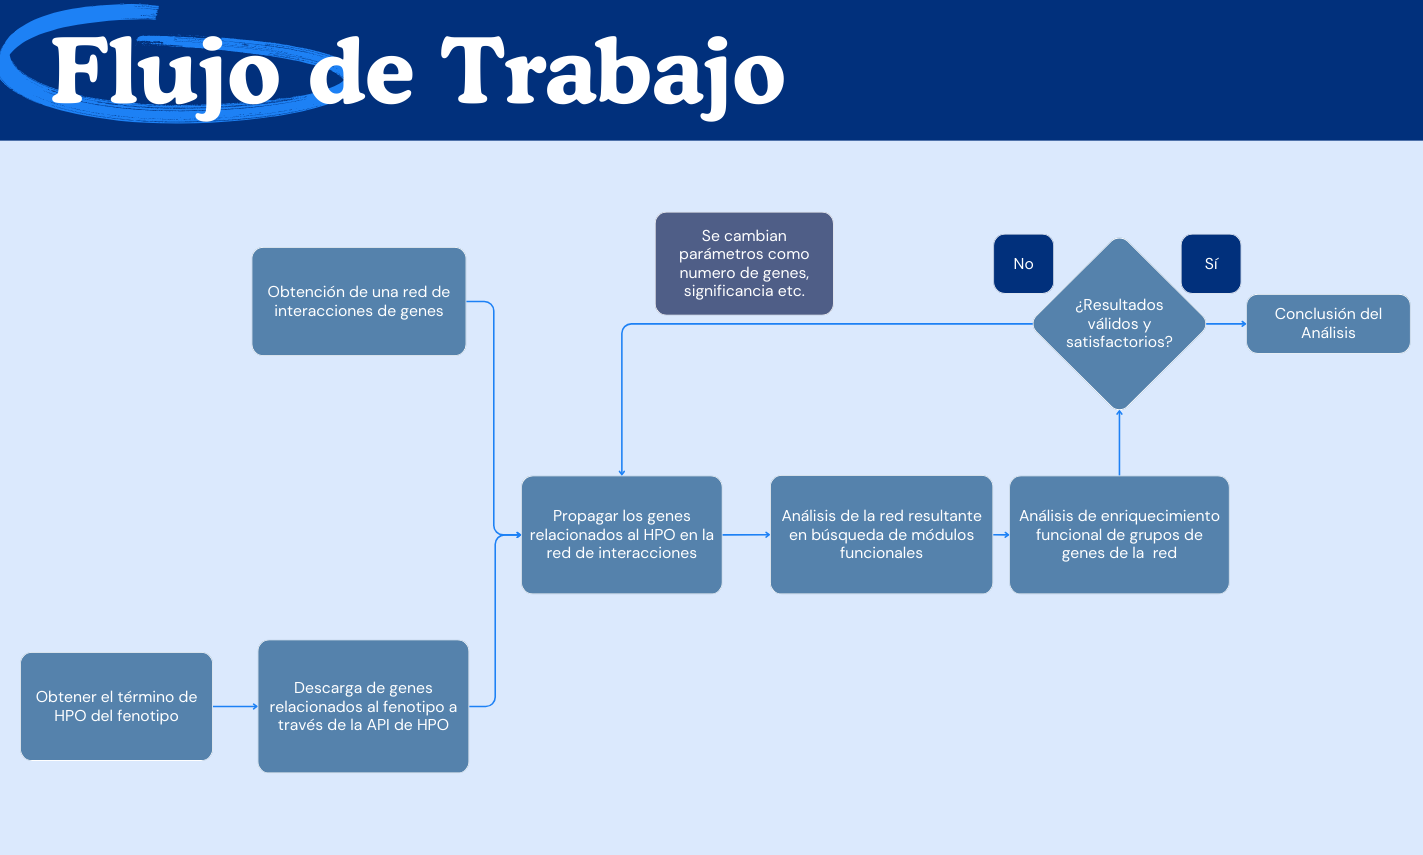
\includegraphics[width=.95\textwidth]{figures/workflow.png}
	\caption{Flujo de trabajo}
	\label{fig:workflow}
\end{figure}

\subsection{Obtención de genes relacionados con signo de Hoffman}

Para obtener los genes relacionados con el signo de Hoffman (HP:0031993), se utilizó la API de la Ontología de Fenotipos Humanos (HPO). En este caso, se emplearon endpoints de la API que devuelven listas tanto de genes (\url{https://ontology.jax.org/api/network/annotation/HP:0031993/download/gene}) como de enfermedades vinculadas al fenotipo de interés (\url{https://ontology.jax.org/api/network/annotation/HP:0031993/download/disease}). Mediante una solicitud HTTP, se extrajo y almacenó esta información en archivos con formato .tsv, facilitando así su posterior análisis. 


\subsection{Obtención de red de interacciones de genes}

Para el análisis de las interacciones génicas, se obtuvo una red de interacciones a partir de la base de datos STRING.

El archivo correspondiente a las interacciones de proteínas humanas (\textit{Homo sapiens}, ID taxonómico: 9606) fue descargado directamente desde \href{https://stringdb-downloads.org/download/protein.links.v12.0/9606.protein.links.v12.0.txt.gz}{el repositorio público de STRING} utilizando un comando en la consola.

Posteriormente, las interacciones fueron filtradas aplicando un umbral mínimo de puntuación combinada (\textit{combined score}) de 700. Posteriormente los identificadores de las proteínas se transformaron a identificadores estándar HUGO.

\subsection{Propagación de red}

Se utilizó el algoritmo DIAMOnD para expandir genes relacionados con el signo de Hoffman en la red de interacciones proteína-proteína. El algoritmo parte de un conjunto inicial de genes de semilla, identificando nodos adicionales cercanos en términos de proximidad topológica, evaluando su conectividad mediante una distribución hipergeométrica. La selección de nodos se basa en su número de conexiones con los genes de semilla, priorizando aquellos que forman una subred coherente, en el proceso biológico del signo de Hoffman. Lo que resultó en una red enriquecida de genes candidatos, visualizados como una subred relacionada con el fenotipo.

\subsection{Análisis de red}
Se aplicó el algoritmo de Louvain para identificar módulos funcionales en la red, agrupando nodos en función de la densidad de sus interacciones. Posteriormente, se calcularon métricas topológicas para analizar la estructura y el rol de los genes en la red. La centralidad de grado permitió identificar nodos con alta conectividad dentro de sus módulos, mientras que la centralidad de intermediación destacó los genes clave en el flujo de información entre módulos. Por último, la centralidad de cercanía ayudó a identificar nodos importantes para la cohesión interna de los módulos.

Este análisis facilitó la identificación de módulos funcionales representados por grupos de genes con posibles relaciones biológicas.

\subsection{Análisis de enriquecimiento funcional}

Una vez identificados los clusters, se realizó un análisis de enriquecimiento funcional para determinar qué funciones biológicas, rutas metabólicas o procesos celulares están sobrerrepresentados en los grupos de genes detectados.
	\section{Resultados}

\subsection{Red de interacción entre genes}

\subsection{Análisis de enriquecimiento funcional}

\subsection{Propiedades de la red y detección de comunidades}

\subsection{Relación de los genes de interés con fenotipos patológicos}
	\section{Discusión}
\subsection{Cluster 1}

\subsubsection{GO Biological Process}

Procesos como el transporte del Golgi a la membrana plasmática (\textit{GO:0006893}) y la organización del cilio (\textit{GO:0044782}) están relacionados con el tráfico vesicular y la señalización celular, esenciales para la dinámica axonal. Estas funciones son cruciales para mantener la integridad de los circuitos neuronales, lo cual podría ser relevante en los reflejos anormales observados en el signo de Hoffman \cite{nachury_ciliary_2010}. Asimismo, el ensamblaje de proyecciones celulares (\textit{GO:0120031}) apunta a un papel en la plasticidad estructural de las neuronas.

\subsubsection{GO Cellular Component}

El endosoma de reciclaje (\textit{GO:0055037}) es clave para la regulación de receptores de membrana, afectando directamente la plasticidad sináptica y el tráfico intracelular neuronal \cite{goldenring_endosome_2019}. Estos procesos son esenciales para la modulación de la actividad sináptica y podrían estar alterados en condiciones de hiperreflexia. Además, el compartimento sensible a insulina (\textit{GO:0032593}) podría influir indirectamente en la regulación del tráfico intracelular en neuronas.

\subsubsection{GO Molecular Function}

La unión a pequeñas GTPasas (\textit{GO:0031267}) y a miosina (\textit{GO:0017022}) subraya la importancia del citoesqueleto en la transmisión neuronal. Alteraciones en estas interacciones podrían comprometer la estructura axonal, lo que es coherente con neuropatías motoras y la disfunción de los reflejos profundos \cite{feiguin_axonal_transport_2001}.

\subsubsection{KEGG Pathways}

La vía de la endocitosis resalta como fundamental en el transporte vesicular y la comunicación neuronal \cite{conner_endocytosis_2003}. Disfunciones en esta ruta pueden alterar la excitabilidad neuronal y contribuir a fenómenos como el signo de Hoffman.




\subsection{Cluster 3}

En la discusión, consideramos apropiado respaldar nuestros resultados citando artículos que vinculan los términos con la neurodegeneración, la cual, como hemos mencionado anteriormente, guarda una estrecha relación con el signo de Hoffman.

\subsubsection{Positive regulation of ATP biosynthetic process - GO Biological Process}
El artículo \cite{Bonvento2017} explica que la regulación positiva del proceso de biosíntesis de ATP está directamente relacionada con la neurodegeneración, ya que las neuronas dependen de una producción eficiente de ATP para mantener los gradientes iónicos esenciales para la transmisión sináptica. La disfunción mitocondrial reduce esta capacidad, lo que provoca la acumulación de daño celular característico de las enfermedades neurodegenerativas. Además, las alteraciones en este proceso intensifican el estrés oxidativo, acelerando el deterioro neuronal y contribuyendo al avance de la enfermedad. 

\subsubsection{Endosome to lysosome transport via multivesicular body sorting pathway - GO Biological Process}
En el artículo \cite{Mulligan2023}, se describe cómo las disfunciones en esta vía de transporte llevan a la acumulación de proteínas mal plegadas y otros desechos celulares en las neuronas. Esta acumulación es una característica común en muchas enfermedades neurodegenerativas, como el Alzheimer y el Parkinson. El estudio utiliza técnicas avanzadas de microscopía para investigar estas interacciones y proporciona un conjunto de enfoques combinatorios para la imagen fija y la imagen en vivo de células, lo que permite una comprensión más profunda de los procesos intracelulares dinámicos.


\subsubsection{Maintenance of synapse structure - GO Biological Process}
En el artículo \cite{Batool2019}, se describe cómo el mantenimiento de la estructura sináptica (GO:0099558) es crucial para la función adecuada del sistema nervioso, y cómo las disfunciones en este proceso pueden llevar a trastornos neurodegenerativos. Se destaca que la formación y el mantenimiento de sinapsis no son estáticos, sino que cambian constantemente para satisfacer las necesidades conductuales del organismo. El estudio utiliza técnicas avanzadas para investigar estos procesos y proporciona una comprensión más profunda de los mecanismos celulares y moleculares involucrados en la formación y el mantenimiento de sinapsis, así como su relación con trastornos neurodegenerativos.

\subsubsection{Mitochondrial intermembrane space - GO Cellular Component}

En el artículo \cite{Kathiresan2024}, se describe cómo las disfunciones en el espacio intermembrana mitocondrial pueden contribuir a la patogénesis de trastornos neurodegenerativos como el Alzheimer, el Parkinson y la enfermedad de Huntington. Se destaca que las mutaciones en el ADN mitocondrial y las alteraciones en la dinámica mitocondrial pueden llevar a una producción de energía comprometida y un aumento del estrés oxidativo, lo que resulta en daño neuronal y muerte celular. El estudio también explora estrategias terapéuticas potenciales dirigidas a la disfunción mitocondrial, incluyendo terapias específicas para mitocondrias y antioxidantes.

\subsubsection{Cytoplasmic stress granule - GO Cellular Component}

En el artículo \cite{10.1093/nar/gkae655}, se describe cómo la formación de gránulos de estrés citoplasmáticos puede mitigar la neurodegeneración. Los gránulos de estrés son complejos de ARN y proteínas que se forman en respuesta a condiciones de estrés celular y juegan un papel crucial en la regulación de la traducción y la supervivencia celular. El estudio utilizó el modelo de la proteína nsP3 del alfavirus para reducir la formación de gránulos de estrés y observó que, en modelos de ataxia, esclerosis lateral amiotrófica y demencia frontotemporal, la reducción de estos gránulos exacerbó los fenotipos de la enfermedad. Esto sugiere que los gránulos de estrés pueden tener un papel protector en las enfermedades neurodegenerativas

En el artículo \cite{PMID:34248597}, se describe cómo los gránulos de estrés citoplasmáticos juegan un papel crucial en la respuesta celular al estrés y su relación con enfermedades neurodegenerativas. Los gránulos de estrés son estructuras sin membrana que se forman en respuesta a condiciones de estrés y ayudan a regular la traducción de ARN y la supervivencia celular. El estudio destaca que la formación y dinámica de estos gránulos están implicadas en la patogénesis de enfermedades como la esclerosis lateral amiotrófica y la demencia frontotemporal, sugiriendo que los gránulos de estrés pueden actuar como precursores de agregados patológicos en estas enfermedades.

\subsubsection{Polyubiquitin modification-dependent protein binding - GO Molecular Function}

En el artículo \cite{Schmidt2021}, se describe cómo la unión de proteínas dependiente de la modificación por poliubiquitina (GO:0031593) juega un papel crucial en la señalización celular y la degradación de proteínas en enfermedades neurodegenerativas. Se destaca que las vías de degradación, como el sistema ubiquitina-proteasoma y la vía autofagia-lisosoma, dependen de la modificación de proteínas con ubiquitina para eliminar proteínas mal plegadas y mantener la salud celular. El estudio también explora cómo la disfunción en estas vías puede llevar a la acumulación de agregados proteicos neurotóxicos, contribuyendo a la patogénesis de enfermedades como el Alzheimer, el Parkinson y la esclerosis lateral amiotrófica.

\subsubsection{K63-linked polyubiquitin modification-dependent protein binding - GO Molecular Function}
En el artículo \cite{10.1093/hmg/ddm320}, se describe cómo la ubiquitinación dependiente de la modificación por poliubiquitina enlazada en K63 (GO:0070530) promueve la formación y la eliminación autofágica de inclusiones proteicas asociadas con enfermedades neurodegenerativas. Se destaca que la ubiquitinación en K63 facilita la acumulación de proteínas y la formación de inclusiones intracelulares, incluso en ausencia de deterioro del proteasoma. Además, esta modificación específica de ubiquitina ayuda a definir el destino de las proteínas para su eliminación a través de la autofagia, proporcionando una ruta mecanística novedosa para el ciclo de vida de los cuerpos de inclusión y ofreciendo potenciales enfoques terapéuticos para tratar trastornos neurodegenerativos.

\subsubsection{Amyotrophic lateral sclerosis (ALS) - KEGG Pathways}

\subsubsection{Mitophagy - KEGG Pathways}

En el artículo \cite{Zhang2022}, se describe cómo la mitofagia, el proceso selectivo de degradación de mitocondrias dañadas o disfuncionales, es crucial para mantener la salud mitocondrial y prevenir la acumulación de mitocondrias defectuosas, lo que es fundamental en la patogénesis de enfermedades neurodegenerativas como el Alzheimer, el Parkinson y la esclerosis lateral amiotrófica. El estudio destaca los mecanismos moleculares que regulan la mitofagia, incluyendo las vías canónicas y no canónicas, y cómo la disfunción en estos procesos puede llevar a la acumulación de mitocondrias dañadas, contribuyendo a la neurodegeneración.
	\section{Conclusiones}

\subsection{Conclusión General}

El análisis identificó interacciones clave entre genes y proteínas relacionadas con el Signo de Hoffmann, detectando grupos funcionales y patrones de interacción potencialmente implicados en procesos neuronales y enfermedades neurodegenerativas, lo que contribuye al entendimiento de sus bases moleculares.

\subsection{Conclusiones Específicas}

\begin{enumerate}
	\item Se identificaron genes relacionados con el Signo de Hoffmann utilizando la Human Phenotype Ontology (HPO) y otras bases de datos relevantes, además de genes que podrían estar indirectamente relacionadas, facilitando la observación de patrones funcionales que no eran evidentes.
	
	\item Se construyó con éxito una red de interacciones proteína-proteína (PPI) destacando nodos relevantes con alta conectividad.
	
	\item Mediante el cálculo de métricas topológicas, se identificaron proteínas clave dentro de la red con potencial importancia en la regulación de procesos neurobiológicos relacionados con la hiperreflexia y la neurodegeneración.
	
	\item El clustering permitió identificar grupos funcionales altamente conectados dentro de la red de interacciones. Estos grupos mostraron correlaciones con procesos biológicos relevantes, como la endocitosis y la regulación del citoesqueleto.
	
	\item El análisis de enriquecimiento funcional confirmó que los genes identificados están involucrados en funciones biológicas críticas, como la regulación de la biosíntesis de ATP y el transporte intracelular, y en vías relacionadas con la neurodegeneración.
\end{enumerate}

\section{Líneas futuras de investigación}

Este estudio abre varias líneas sobre los mecanismos moleculares del Signo de Hoffmann y su relación con enfermedades neurogenerativas. Sería enriquecedor validar las interacciones propuestas mediante estudios experimentales e integrar nuevos datos para un análisis más completo.

\begin{itemize}
	\item Validación experimental de las interacciones proteína-proteína identificadas en modelos celulares o animales.
	\item Exploración de las modificaciones postraduccionales de proteínas clave involucradas en los procesos identificados.
	\item Ampliación del análisis a otras patologías relacionadas con hiperreflexia para identificar posibles conexiones comunes.
	\item Análisis longitudinal de la expresión de los genes identificados en diferentes etapas de la neurodegeneración.
	\item Integración de datos ómicos adicionales (transcriptómica, epigenómica) para un análisis más exhaustivo de las redes moleculares implicadas.
\end{itemize}


	
	
	%%%%%%%%%%%%%%%%%%%%%%%%%%%%%%%%%%%%%%%%%%%%%%
	%% OTRA INFORMACIÓN                         %%
	%%%%%%%%%%%%%%%%%%%%%%%%%%%%%%%%%%%%%%%%%%%%%%
	
	\begin{backmatter}
	
		\section*{Abreviaciones}%% if any
		\begin{itemize}
			\item \textbf{HPO}: Human Phenotype Ontology, En español: La ontología del fenotipo humano.
			\item \textbf{OMIM}: Online Mendelian Inheritance in Man, En español: Herencia mendeliana en línea en el hombre.
			\item \textbf{ELA}: esclerosis lateral amiotrófica.
		\end{itemize}
		
		\section*{Disponibilidad de datos y materiales}%% if any
			% Texto original: Debéis indicar aquí un enlace a vuestro repositorio de github.
			
			
			Puedes encontrar más información en el \href{https://github.com/Diegodepab/project_template}{repositorio de github}
			 
			
		\section*{Contribución de los autores}
			Usando las iniciales que habéis definido al comienzo del documento, debeis indicar la contribución al proyecto en el estilo:
			J.E : Encargado del análisis de coexpresión con R, escritura de resultados; J.R.S : modelado de red con python y automatizado del código, escritura de métodos; ...
			OJO: que sea realista con los registros que hay en vuestros repositorios de github. 
		
		
		%%%%%%%%%%%%%%%%%%%%%%%%%%%%%%%%%%%%%%%%%%%%%%%%%%%%%%%%%%%%%%%%%%%%%%%%%%%%%%%%%%%%%%%%
		%% BIBLIOGRAFIA: no teneis que tocar nada, solo sustituir el archivo bibliography.bib %%
		%% por el que hayais generado vosotros                                                %%
		%%%%%%%%%%%%%%%%%%%%%%%%%%%%%%%%%%%%%%%%%%%%%%%%%%%%%%%%%%%%%%%%%%%%%%%%%%%%%%%%%%%%%%%%
		
		\bibliographystyle{bmc-mathphys} % Style BST file (bmc-mathphys, vancouver, spbasic).
		\bibliography{bibliography}      % Bibliography file (usually '*.bib' )
	
	\end{backmatter}
\end{document}
